\documentclass[letterpaper,11pt]{article}
\usepackage{etex}
\usepackage{enumitem}
\reserveinserts{28}
\usepackage{amssymb}
\usepackage{theorem}
%\usepackage{savetrees}
\usepackage[margin=2cm]{geometry}
\usepackage{graphicx}
\usepackage{fancybox}
\usepackage{fancyhdr}
\usepackage{tabularx}
\usepackage{color}
\usepackage{xcolor}
\usepackage{multirow}
\usepackage{amsmath}
\usepackage[utf8]{inputenc} % Pour pouvoir taper les accent directement et non pas passer par \'
\usepackage[T1]{fontenc} %%% Pour que les accents soient correctement traités dans le PDF et le DVI
\usepackage{lmodern} %Un autre package pour les accents français
\usepackage[french]{babel} %Un autre package pour les accents
\usepackage{ifthen}
%\usepackage{multicol}
%\usepackage{cancel}
\usepackage{pst-all}
\usepackage{pstricks-add}
\usepackage{multicol}
%\usepackage{tikz}
%\usepackage{pgf,tikz}
%\usepackage{circuitikz}
%\usetikzlibrary{shapes}
%\usetikzlibrary{calc}
%\usetikzlibrary{plotmarks}
%\usepackage{tkz-fct}
\usepackage{fp}
\usepackage{float}
\usepackage{siunitx}
\usepackage{pdfpages}%Pour sortir seulement certaine pages du pdf
\usepackage{textcomp}
\usepackage{hyperref}
\hypersetup{
    colorlinks=true, % make the links colored
    linkcolor=blue, % color TOC links in blue
    urlcolor=red, % color URLs in red
    linktoc=all % 'all' will create links for everything in the TOC
}

\sisetup{locale = FR, number-math-rm, per-mode=symbol, separate-uncertainty}

\renewcommand{\exp}[1]{\mathrm{e}^{#1}}

\setlength{\parindent}{0pt}



\begin{document}


\begin{center}
~
\vfill
\LARGE{Travail Pratique 2 (IFT-4201/IFT-7201)}\\[0.4cm]

\Large{Présenté à Audrey Durand}

\vfill
\large{Équipe 10: Adam Cohen, Maxime Genest, Vincent Masse}

\vfill
\thispagestyle{empty}

\end{center}

\clearpage

\pagestyle{fancy}
\lhead{IFT-7201}
\chead{Devoir 2 (Automne 2020)}
\rhead{Équipe 10}

\section{Deep $Q$-learning}

\begin{enumerate}[label=(\alph*)]

\item \textbf{État comme seule entrée}\\
La fonction prenant en entrée seulement l'état permet d'avoir plus de flexibilités.
Avec cette fonction, il est possible d'avoir des poids différents pour chaque action, ce qui n'est pas possible avec la fonction qui prend en entrée (état-action). En effet, avec la fonction état-action, on peut seulement ajouter des paramètres qui modifiera la sortie pour la valeur Q, alors que pour la fonction qui prend seulement l'état en entrée, on a des poids différent pour chaque action.

\item \textbf{Réseau cible}\\
L'oubli catastrophique est le fait qu'un réseau de neurones oubli son apprentissage lorsqu'il doit apprendre une nouvelle tâche, c'est un peu comme s'il recommençait son apprentissage à 0. Le fait de fixer les poids $\theta$ dans la cible pendant plusieurs mise à jours permet de conserver une certaine stabilité pour permettre la convergence.

\item \textbf{Heuristique}\\
Si $\tau$ est trop grand, la cible est trop modifié, ce qui risque de compromettre la convergence (voir numéro précédent), le cas limite $\tau=1$ revient à ne pas fixer (même pas partiellement) les targets. Si $\tau$ est trop petit, les targets seront trop fixes, et donc les cibles ne sont pratiquement pas améliorées et le réseau apprend donc sur des moins bonnes cibles (non-représentative de ce que l'on doit viser). Le cas limite $\tau=0$ montre un cas où la cible n'est jamais modifiée et gardera toujours sa valeur initiale, ce qui est bien entendu non-souhaitable. 

\item \textbf{Replay buffer}\\
L'avantage de son utilisation est de briser la corrélation entre les échantillons utilisés lors de la mise à jour (le tuple $(s_t, a_t, r_{t+1}, s_{t+1})$ et le tuple suivant $(s_{t+1}, a_{t+1}, r_{t+2}, s_{t+2})$ partage le même état $s_{t+1}$). Cela compromet l'apprentissage. Le fait de stocker les échantillons et d'échantillonner une mini-batch plusieurs fois au cours de l'épisode permet contourner ce problème. À COMPLÉTER  

\item \textbf{Apprentissage supervisée}\\


\item Parmi les défis d'implémentations auxquels on a fait face, l'un d'entre eux et la longueur d'un entraînement, cela a fait en sorte qu'il était difficile de tester différents paramètres d'entraînements et d'optimiser cette dernières. Une ressource de calcul plus puissante que nos ordinateurs personnels aurait sans doute permis de faire un plus large éventail de tests. Voici deux graphiques illustrant l'évolution des gains épisodiques durant l'entraînement ainsi que l'évolution épisodique de la fonction de perte.

\begin{center}
\begin{figure}[H]
\caption{Évolution des gains et fonction de pertes}
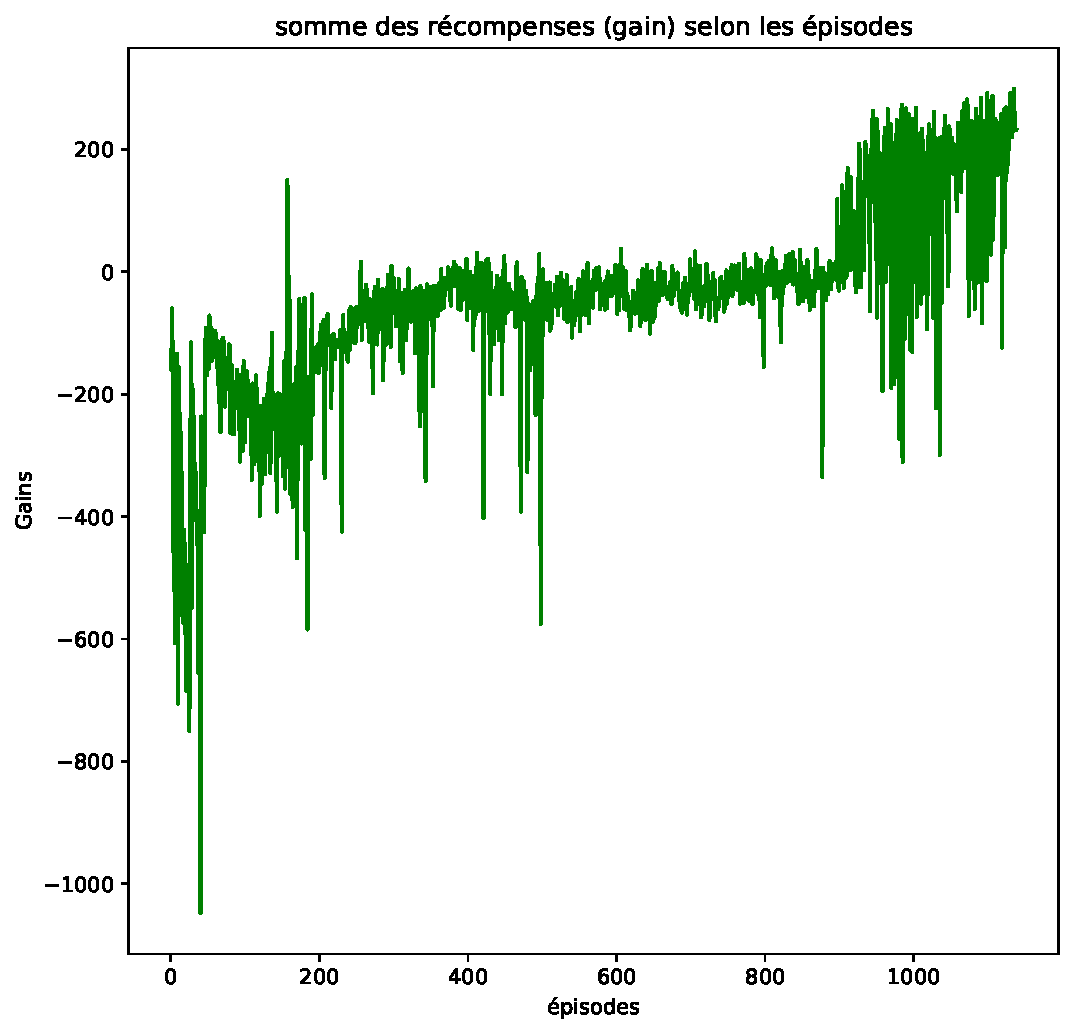
\includegraphics[width=0.45\linewidth]{gains.pdf} \hfill 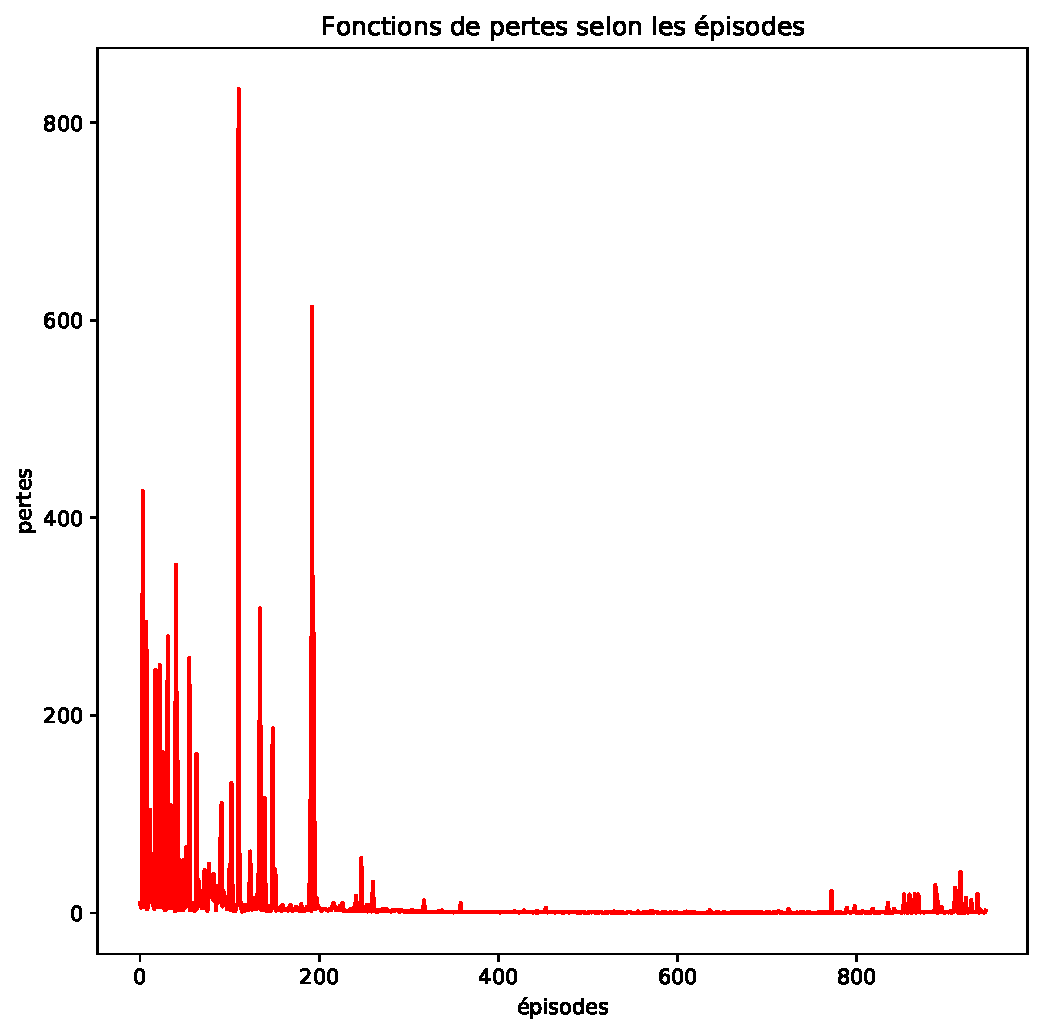
\includegraphics[width=0.45\linewidth]{pertes.pdf}
\end{figure}
\end{center}

FONCTION DE PERTE CI-DESSUS À MODIFIER (Je ne suis pas certain que c'est ça qu'il est demandé)

Voici maintenant le graphique de la fonction de gain par pas de temps dans l'environnement pour un épisode joué par notre agent entraîner (donc par la politique apprise).
 
\begin{figure}[H]
\begin{center}
\caption{}
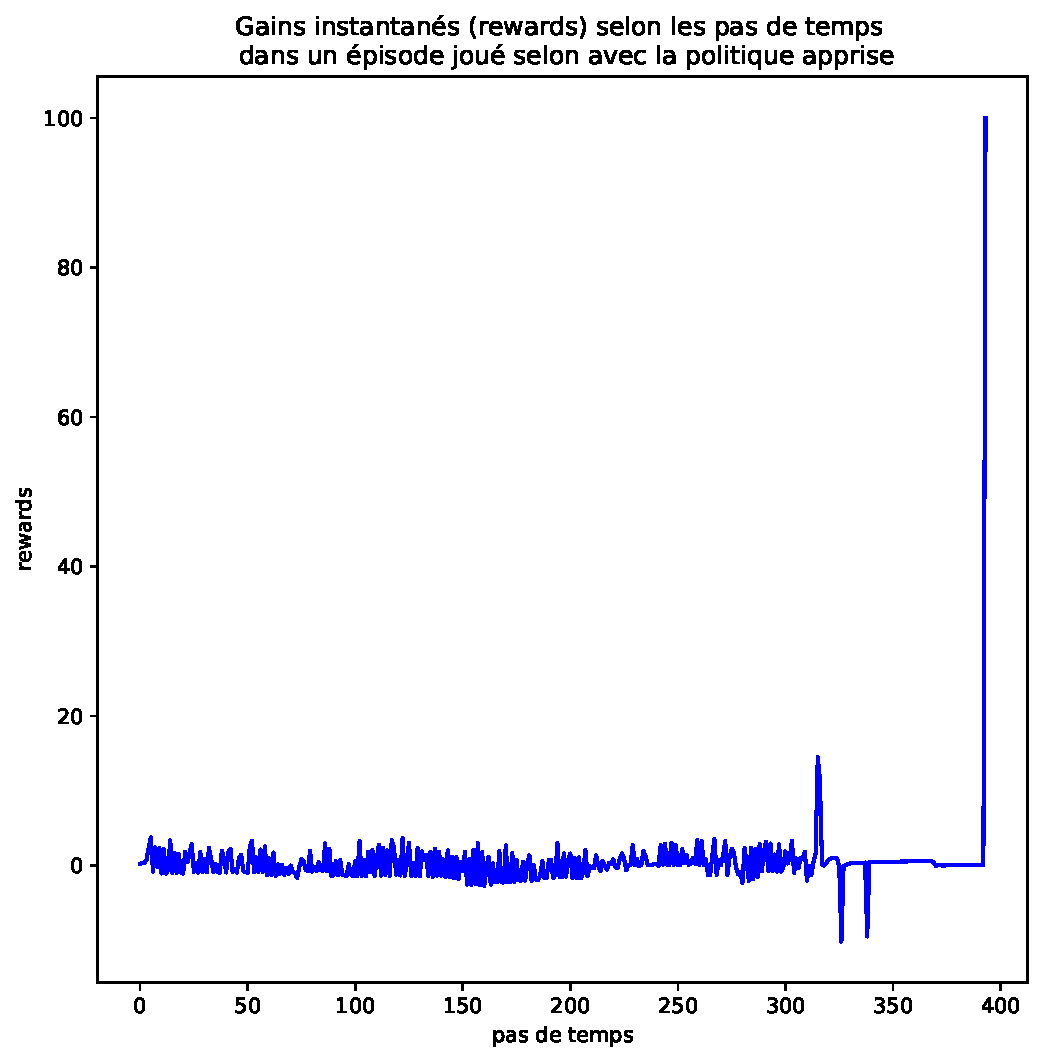
\includegraphics[scale=0.5]{gain_par_pas.pdf}
\end{center}
\end{figure}

\end{enumerate}

\section{SARSA}

\begin{enumerate}[label=(\alph*)]

\item \textbf{Exploration}\\
L'initialisation de la fonction de valeurs d'actions est associée à l'initialisation des estimateurs empiriques des actions dans l'approche des bandits. Dans cet environnement, puisque l'on initialise les $Q(s,a)=0$ et que la fonction de reward donne un reward de $-1$ à toutes les actions ou l'auto n'atteint pas le drapeau, cela revient à faire une initialisation optimiste de l'estimateur. En effet, en initialisant tous les $Q_{vals}=0,$ toutes les actions essayées feront pire que les actions dont la valeur est encore la valeur initiale, ainsi cela force l'algorithme à essayer les autres actions possibles.

\item

\end{enumerate}

\end{document}
